\subsection{Inner Tracker}
The inner tracker is designed to perform precise measurements of charged-particle trajectories and precise reconstruction of secondary vertices originating from the decay of tau leptons and long-lived hadrons. It surrounds the interaction point and has a length of 5.8~\unit{m} and a diameter of 2.5~\unit{m}. Silicon-based detector technology was chosen for its great granularity, fast response, and reasonable radiation hardness. The tracker is divided into two main components: the pixel detector, which is closest to the interaction point, and the strip tracker, which surrounds the pixel detector. \Cref{fig:tracker} shows a sketch of one quarter of the inner tracker.

Originally, the pixel detector consisted of three barrel layers at $r=$ 4.4~\unit{cm}, 7.3~\unit{cm} and 10.2~\unit{cm}, and two forward/backwards disks at $\abs{z}=$ 34.5~\unit{cm} and 46.5~\unit{cm}, extending in radius from about 6~\unit{cm} to 15~\unit{cm}. In total, the pixel detector had 66 million pixels, covering an area of 1.06~\unit{m^2}~\cite{CMS:2008xjf}. To accommodate higher luminisoties, the pixel detector was upgraded with increased granularity in the end-of-year technical stop of the LHC in 2016/2017~\cite{CMS:2012sda}. The new pixel detector consists of four barrel layers at $r=$ 2.9~\unit{cm}, 6.8~\unit{cm}, 11~\unit{cm}, and 16~\unit{cm}, and three forward/backwards disks at $\abs{z}=$ 29~\unit{cm}, 40~\unit{cm}, and 52~\unit{cm}, extending in radius from 4.5~\unit{cm} to 16.1~\unit{cm}. In total, the upgraded pixel detector has 124 million pixels, of size 100~\unit{\micro m} $\times$ 150~\unit{\micro m}, covering a total area of 1.9~\unit{m^2}~\cite{CMSTrackerGroup:2020edz}. This geometry is designed to measure four space points (hits) along a charged particle's trajectory, in the pseudorapidity range $\abs{\eta} < 2.5$. This results in a spatial resolution of 12~\unit{\micro m} in the transverse ($r$-$\phi$) plane, and 22~\unit{\micro m} in the longitudinal ($z$) direction~\cite{CMSTrackerGroup:2020edz}.

\begin{figure}
  \centering
  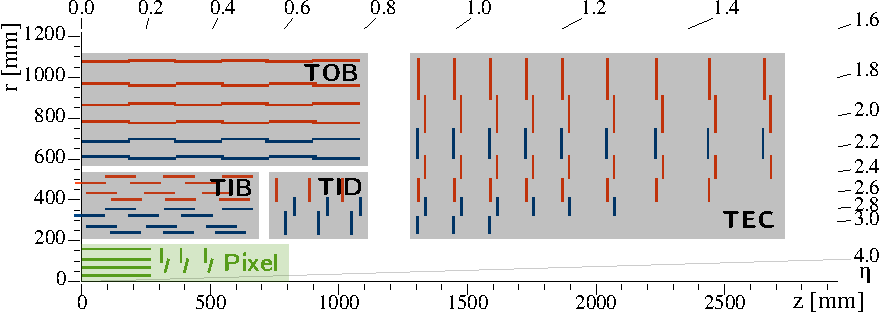
\includegraphics[width=\textwidth]{Figures/Detector/CMS/tracker_annotated.pdf}
  \caption[The CMS Inner Tracker]{Sketch of one quarter of the CMS inner tracker after the 2016/2017 upgrade in the r-z plane. The pixel detector is shown in green, while the single-sided and double-sided strip modules are shown in red and blue respectively. Figure adapted from Ref.~\cite{CMS:2017lum}.}\label{fig:tracker}
\end{figure}

At radii between 20~\unit{cm} and 116~\unit{cm}, lower occupancies allow for the use of strip detectors. The strip tracker consists of three subsystems. The Tracker Inner Barrel and Disks (TIB/TID) subsystem comprises four barrel layers and three forward/backward disks which extend to a radius of 55~\unit{cm} and use 320~\unit{\micro m} thick silicon microstrip sensors. Depending on the layer, the strip pitch\footnote{Strip pitch refers to the centre-to-centre distance between adjacent strips} is 80--141~\unit{\micro m} in the TIB/TID. With the strips laying parallel to the beam axis in the TIB, and radially in the TID, the TIB/TID provides up to 4 $\phi$ measurements per track, leading to a spatial resolution in $r\phi$ of 23--35~\unit{\micro m}. Extending to a radius of 116~\unit{cm}, the Tracker Outer Barrel (TOB) subsystem consists of six barrel layers, which use 500~\unit{\micro m} thick silicon microstrip sensors with a pitch of 122--183~\unit{\micro m}. The TOB provides up to 6 $\phi$ measurements per track, leading to a spatial resolution in $r\phi$ of 35--53~\unit{\micro m}. 

The TID/TIB and TOB subsystems extend to $\abs{z} = 118~\unit{cm}$. Beyond this are the Tracker EndCaps (TEC), which extend to $\abs{z} = 282~\unit{cm}$ and cover $22.5 < \abs{r} < 113.5~\unit{cm}$. Each endcap consists of nine disks, with up to 7 rings of silicon strip detectors of 320~\unit{\micro m} thickness for the inner 4 rings, and 500~\unit{\micro m} thickness for the outer 3 rings with radial strips of 97--184~\unit{\micro m} pitch. Therefore, they provide up to 9 measurements of $\phi$ per track.

Finally, the first two layers and rings of the TIB, TID and TOB, as well as rings 1,2 and 5 of the TECs are fitted with a second strip detector module which is mounted back to back with the first module. These modules have their strips rotated at an almost perpendicular angle to the first module, and therefore provide a measurement of a second coordinate, that being $z$ in the barrel and $r$ on the disks. The spatial resolution of these measurements are 230~\unit{\micro m} and 530~\unit{\micro m} in the TIB and TOB respectively, and varies with pitch in the TID and TEC.

This tracker layout ensures at least $\approx 9$ hits per trajectory in the silicon strip tracker for $\abs{\eta} < 2.4$, with the ultimate acceptance of the tracker ending at $\abs{\eta} = 2.5$. In total, the strip tracker has 9.3 million strips and 198~\unit{m^2} of active silicon area~\cite{CMS:2008xjf}.